\textbf{Q3. Games} \\

\begin{enumerate}
\item {\bf Games.} 
Consider the game tree below, which contains maximizer nodes, minimizer nodes, and chance nodes.  For the chance nodes the probability of each outcome is equally likely.

\begin{enumerate}
	\item  Fill in the values of each of the nodes. [10 pts] \\[3mm]

	\item Is pruning possible? [10 pts] \\[1mm]
	\begin{enumerate}
		\item No.  Brief justification: \\
		\item Yes.  Cross out the branches that can be pruned.
	\end{enumerate}
     

\end{enumerate}

\begin{center}
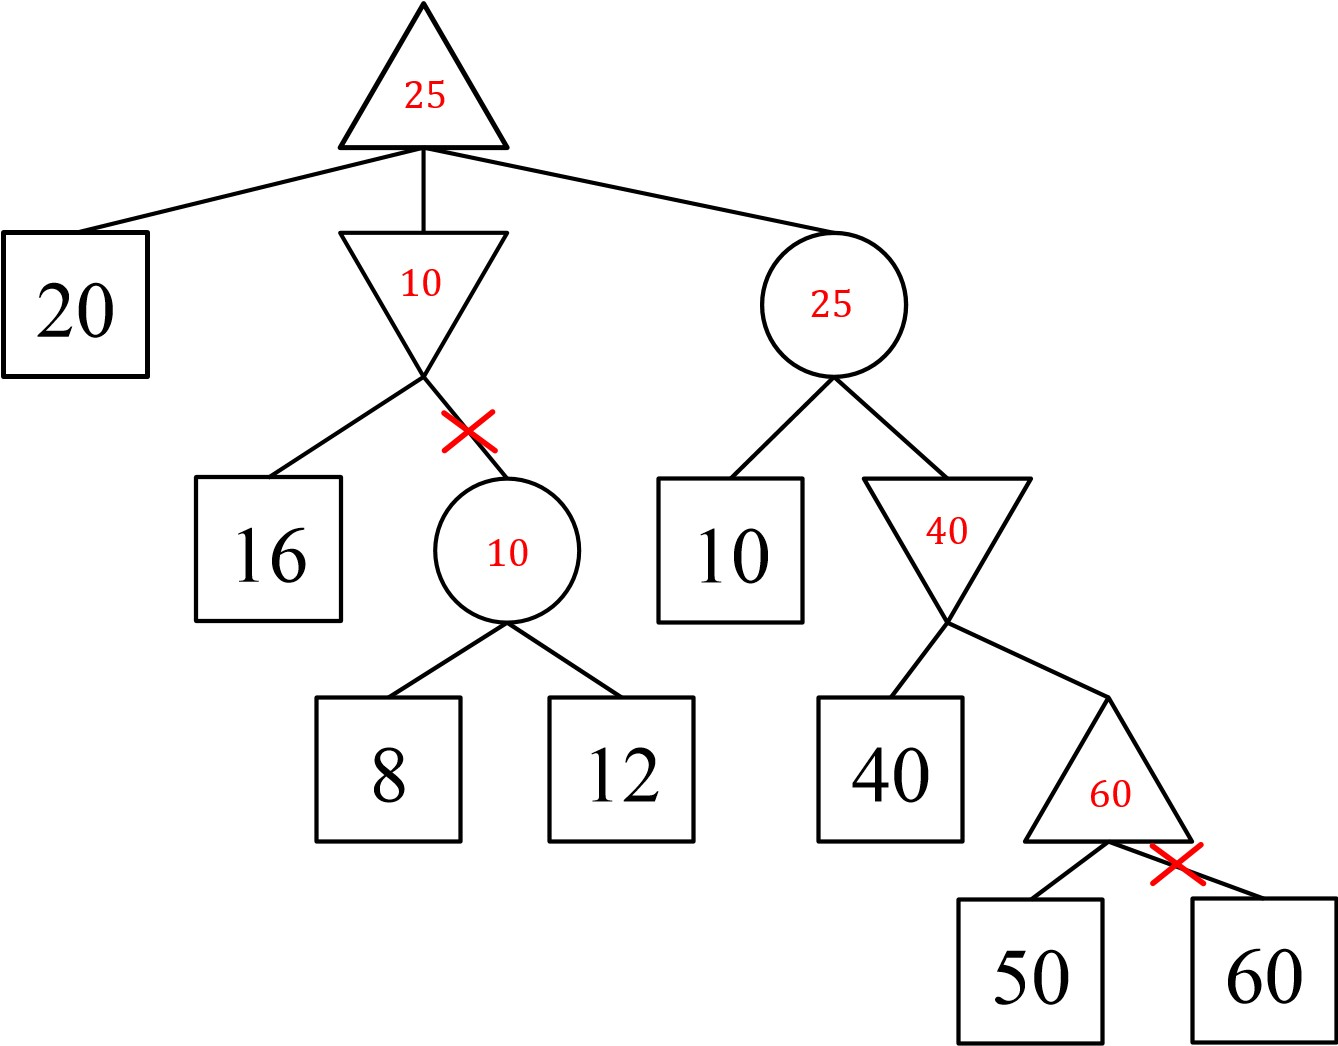
\includegraphics[width=0.71\linewidth]{figures/short-questions-games_sol.jpg}
\end{center}



\item {\bf Utilities.} Pacman's utility function is $U(\$ x) = \sqrt{x}$.  He is faced with the following lottery: $[0.5, \$ 36 \ ; \ 0.5, \$ 64]$. What is Pacman's expected utility? [10 pts]

{ \color{red}
The utility of a lottery can be computed via $EU(L) = \sum_{x \in L} p(x) U(x)$ \\
Hence, $EU( [0.5, \$ 36 \ ; \ 0.5, \ \$ 64]) = 0.5 U( \$36) + 0.5 U( \$64) = 0.5 (6) + 0.5 (8) = 7$
}


\end{enumerate}